\newcommand{\ClassPath}{../VIU_TFM_LaTeX_template}
\documentclass{\ClassPath/viu-tfm-template}
\usepackage{multicol}

\definecolor{maincolor}{HTML}{f25416}

%--------------------------------------------------------------------------
% Definiciones necesarias Modifica con tus datos
%--------------------------------------------------------------------------
\def\nombre{Gómez Olivencia, Rubén}
\def\dni{78910013-A}
\def\titulo{Product backlog y Sprint backlog}
\def\titulacion{Máster Universitario en Desarrollo de Aplicaciones y Servicios Web}
\def\curso{2022-2023}

%Los siguientes son opcionales: si no se ponen, la portada cambia un poco. Ideal para escribir artículos/trabajos cortos
\def\dirige{}
\def\convocatoria{}
\def\asignatura{Gestión de proyectos en entornos ágiles}


% importar fichero de Bibliografía
%\addbibresource{Actividad_1.bib}

\begin{document}
    \graphicspath{{../VIU_TFM_LaTeX_template/}}

    \coverpage

    \tableofcontents

\chapter{Introducción}

Hoy en día es conveniente hacer uso de las \textbf{metodologías ágiles} cuando realizamos la gestión de un proyecto, ya que cuentan con una serie de ventajas que nos van a permitir dar una respuesta más rápida y flexible ante posibles cambios durante la vida de desarrollo del producto.

Las metodologías ágiles cuentan con una serie de ventajas entre las que podemos destacar:

\begin{itemize}
    \item Podremos entregar resultados funcionales al cliente cada poco tiempo y así obtener \textit{feedback} de lo realizado.
    \item Seremos capaces de dar una respuesta ágil y flexible ante posibles cambios que puedan surgir (cambios en los requisitos, ante bajas de personal asignado al proyecto, dificultades durante el desarrollo...).
    \item Tratar de evitar burocracia innecesaria, para centrarnos de esta manera en el producto y sus funcionalidades.
    \item Se trata de involucrar al cliente y colaborar con él para de esta manera conseguir un mayor valor al producto.
\end{itemize}

Con todo ello, se va a realizar la gestión de un proyecto que dará como resultado un gestor de contraseñas y documentación sensible basado en una plataforma web creada con \href{https://angular.io/}{Angular} y que hará uso como backend del sistema \href{https://www.vaultproject.io/}{Vault} de la empresa Hashicorp.


\chapter{Historias de usuario}

Para comenzar con la gestión del proyecto debemos obtener los requisitos del cliente y transformarlos en las conocidas como “\textbf{historias de usuario}”.

En ellas plasmaremos, en un lenguaje que pueda entender el cliente, las funcionalidades que el producto debe tener, a las que asociaremos otros datos como son:

\begin{itemize}
    \item \textbf{Identificador único} para poder diferenciarlas del resto.
    \item Una \textbf{estimación de tiempos}
    \item \textbf{Prioridad} inicial para poder ordenarlas entre ellas.
    \item Se asignará a un desarrollador.
    \item Se añadirán posibles dependencias de otras historias de usuario.
    \item Una \textbf{descripción} de lo que se quiere conseguir.
    \item Unos \textbf{criterios de validación} por parte del cliente.
\end{itemize}

\section{Resultado del análisis realizado}

A continuación se van a plasmar las distintas “historias de usuario” obtenidas:

\begin{requisitostbl}{X[-1]X[-1]X[-1]X[1]X[-1]}
    ID & Estimación & Prioridad  & Asignación &  Dependencias \\
    1  & 15 horas & 1  & Ariane Olivencia &   \\

    Desarrollar “esqueleto” del interfaz web \\

    \textbf{Descripción}:
    Como usuario necesito un interfaz web para poder acceder a la aplicación y hacer uso de ella. Es la base del proyecto. \\

    \textbf{Criterios de validación}:
    El interfaz es responsive, visualmente atractivo y funcional. \\
\end{requisitostbl}

\begin{requisitostbl}{X[-1]X[-1]X[-1]X[1]X[-1]}
    ID & Estimación & Prioridad  & Asignación &  Dependencias \\
    2  & 5 horas & 1  & Rubén Gómez & 1  \\

    Crear login de usuario \\

    \textbf{Descripción}:
    Como usuario quiero poder acceder a la aplicación utilizando como sistema de autenticación un usuario y contraseña.  \\

    \textbf{Criterios de validación}:
    Los valores introducidos serán autenticados contra el \textit{backend} que el cliente decida (base de datos o LDAP/Active Directory). \\
\end{requisitostbl}


\begin{requisitostbl}{X[-1]X[-1]X[-1]X[1]X[-1]}
    ID & Estimación & Prioridad  & Asignación &  Dependencias \\
    3  & 30 horas & 1  & Rafael Gómez & 2  \\

    Listado de secretos \\

    \textbf{Descripción}:
    Como usuario quiero poder obtener un listado de los secretos existentes para poder navegar por ellos y seleccionar el que me interese. \\

    \textbf{Criterios de validación}:
    \begin{itemize}
        \item El listado completo se obtiene mediante un árbol jerarquizado.
        \item Se puede navegar por el árbol seleccionando “directorios” que desplegarán a su vez su contenido.
        \item También se puede hacer como si fuera un explorador de archivos.
        \item Se puede buscar por el nombre de los secretos.
    \end{itemize}
    \\
\end{requisitostbl}

\vspace{20pt}

\begin{requisitostbl}{X[-1]X[-1]X[-1]X[1]X[-1]}
    ID & Estimación & Prioridad  & Asignación &  Dependencias \\
    4  & 10 horas & 2  & Carmen Olivencia & 2  \\

    Visualizar un secreto \\

    \textbf{Descripción}:
    Como usuario quiero acceder a un secreto para visualizar su contenido.  \\

    \textbf{Criterios de validación}:
    \begin{itemize}
        \item La visualización mostrará el secreto en formato HTML.
        \item Si un usuario accede a un secreto “bloqueado” lo debe saber y no se le permitirá editarlo.
        \item Al visualizar el secreto aparecerán botones con distintas acciones que se podrán realizar sobre él (editar, imprimir, ver históricos, borrar).
    \end{itemize}
    \\
\end{requisitostbl}


\begin{requisitostbl}{X[-1]X[-1]X[-1]X[1]X[-1]}
    ID & Estimación & Prioridad  & Asignación &  Dependencias \\
    5  & 25 horas & 2  & Rubén Gómez & 2  \\

    Modificar un secreto \\

    \textbf{Descripción}:
    Como usuario quiero poder editar un secreto para realizar modificaciones.  \\

    \textbf{Criterios de validación}:
    \begin{itemize}
        \item La modificación se realizará a través de un editor \textit{\textbf{WYSIWYG}}.
        \item El editor permitirá realizar modificaciones en formato \href{https://es.wikipedia.org/wiki/Markdown}{Markdown}.
        \item El editor permitirá guardar el secreto y al hacerlo volveremos a la visualización del mismo.
        \item Al comenzar la modificación el secreto se pondrá en estado “bloqueado”.
    \end{itemize}
    \\
\end{requisitostbl}

\vspace{10pt}

\begin{requisitostbl}{X[-1]X[-1]X[-1]X[1]X[-1]}
    ID & Estimación & Prioridad  & Asignación &  Dependencias \\
    6  & 10 horas & 3  & Asier Gómez & 4  \\

    Borrado de secretos \\

    \textbf{Descripción}:
    Como usuario quiero poder borrar secretos para que desaparezcan.  \\

    \textbf{Criterios de validación}:
    Antes de borrar debe existir un mensaje de confirmación. \\
\end{requisitostbl}

\vspace{10pt}

\begin{requisitostbl}{X[-1]X[-1]X[-1]X[1]X[-1]}
    ID & Estimación & Prioridad  & Asignación &  Dependencias \\
    7  & 15 horas & 3  & Ariane Olivencia & 2  \\

    Permitir gestionar ficheros como secretos \\

    \textbf{Descripción}:
    Como usuario quiero poder subir ficheros al sistema para guardarlos cifrados.  \\

    \textbf{Criterios de validación}:
    Se permite subir cualquier tipo de fichero y se podrá descargar. Se debe poder visualizar los ficheros más habituales en la propia web (imágenes y ficheros PDF) sin necesidad de descargarlos. \\
\end{requisitostbl}





\begin{requisitostbl}{X[-1]X[-1]X[-1]X[1]X[-1]}
    ID & Estimación & Prioridad  & Asignación &  Dependencias \\
    8  & 20 horas & 4  & Rafael Gómez & 4  \\

    Versionado de secretos\\

    \textbf{Descripción}:
    Como usuario quiero poder ver las veces que el fichero ha sido modificado para poder ver los cambios realizados.  \\

    \textbf{Criterios de validación}:
    \begin{itemize}
        \item Poder ver el número de versiones que tiene un secreto.
        \item Poder ver una versión concreta del secreto.
        \item Poder ver las diferencias entre versiones.
        \item Poder restaurar una versión conrecta del secreto.
    \end{itemize} \\
\end{requisitostbl}






\begin{requisitostbl}{X[-1]X[-1]X[-1]X[1]X[-1]}
    ID & Estimación & Prioridad  & Asignación &  Dependencias \\
    9  & 5 horas & 4  & Asier Gómez & 2  \\

    Imprimir secretos \\

    \textbf{Descripción}:
    Como usuario quiero poder imprimir un secreto. \\

    \textbf{Criterios de validación}:
    Existe un botón para imprimir un secreto. \\
\end{requisitostbl}



\begin{requisitostbl}{X[-1]X[-1]X[-1]X[1]X[-1]}
    ID & Estimación & Prioridad  & Asignación &  Dependencias \\
    10  & 35 horas & 2  & Rubén Gómez & 1  \\

    Puesta en producción segura \\

    \textbf{Descripción}:
    Como usuario quiero poder acceder a la plataforma de manera segura para realizar todo lo comentado hasta ahora \\

    \textbf{Criterios de validación}:
    \begin{itemize}
        \item El acceso web tiene que ser por HTTPS (certificado válido).
        \item El servidor debe estar securizado ante accesos externos.
        \item Los servicios deben auto-arrancarse en caso de caída.
        \item Existe un registro de lo sucedido a cada secreto (auditoría).
    \end{itemize} \\
\end{requisitostbl}


\section{Mapa de las historias de usuario}

Para visualizar

\begin{center}
    %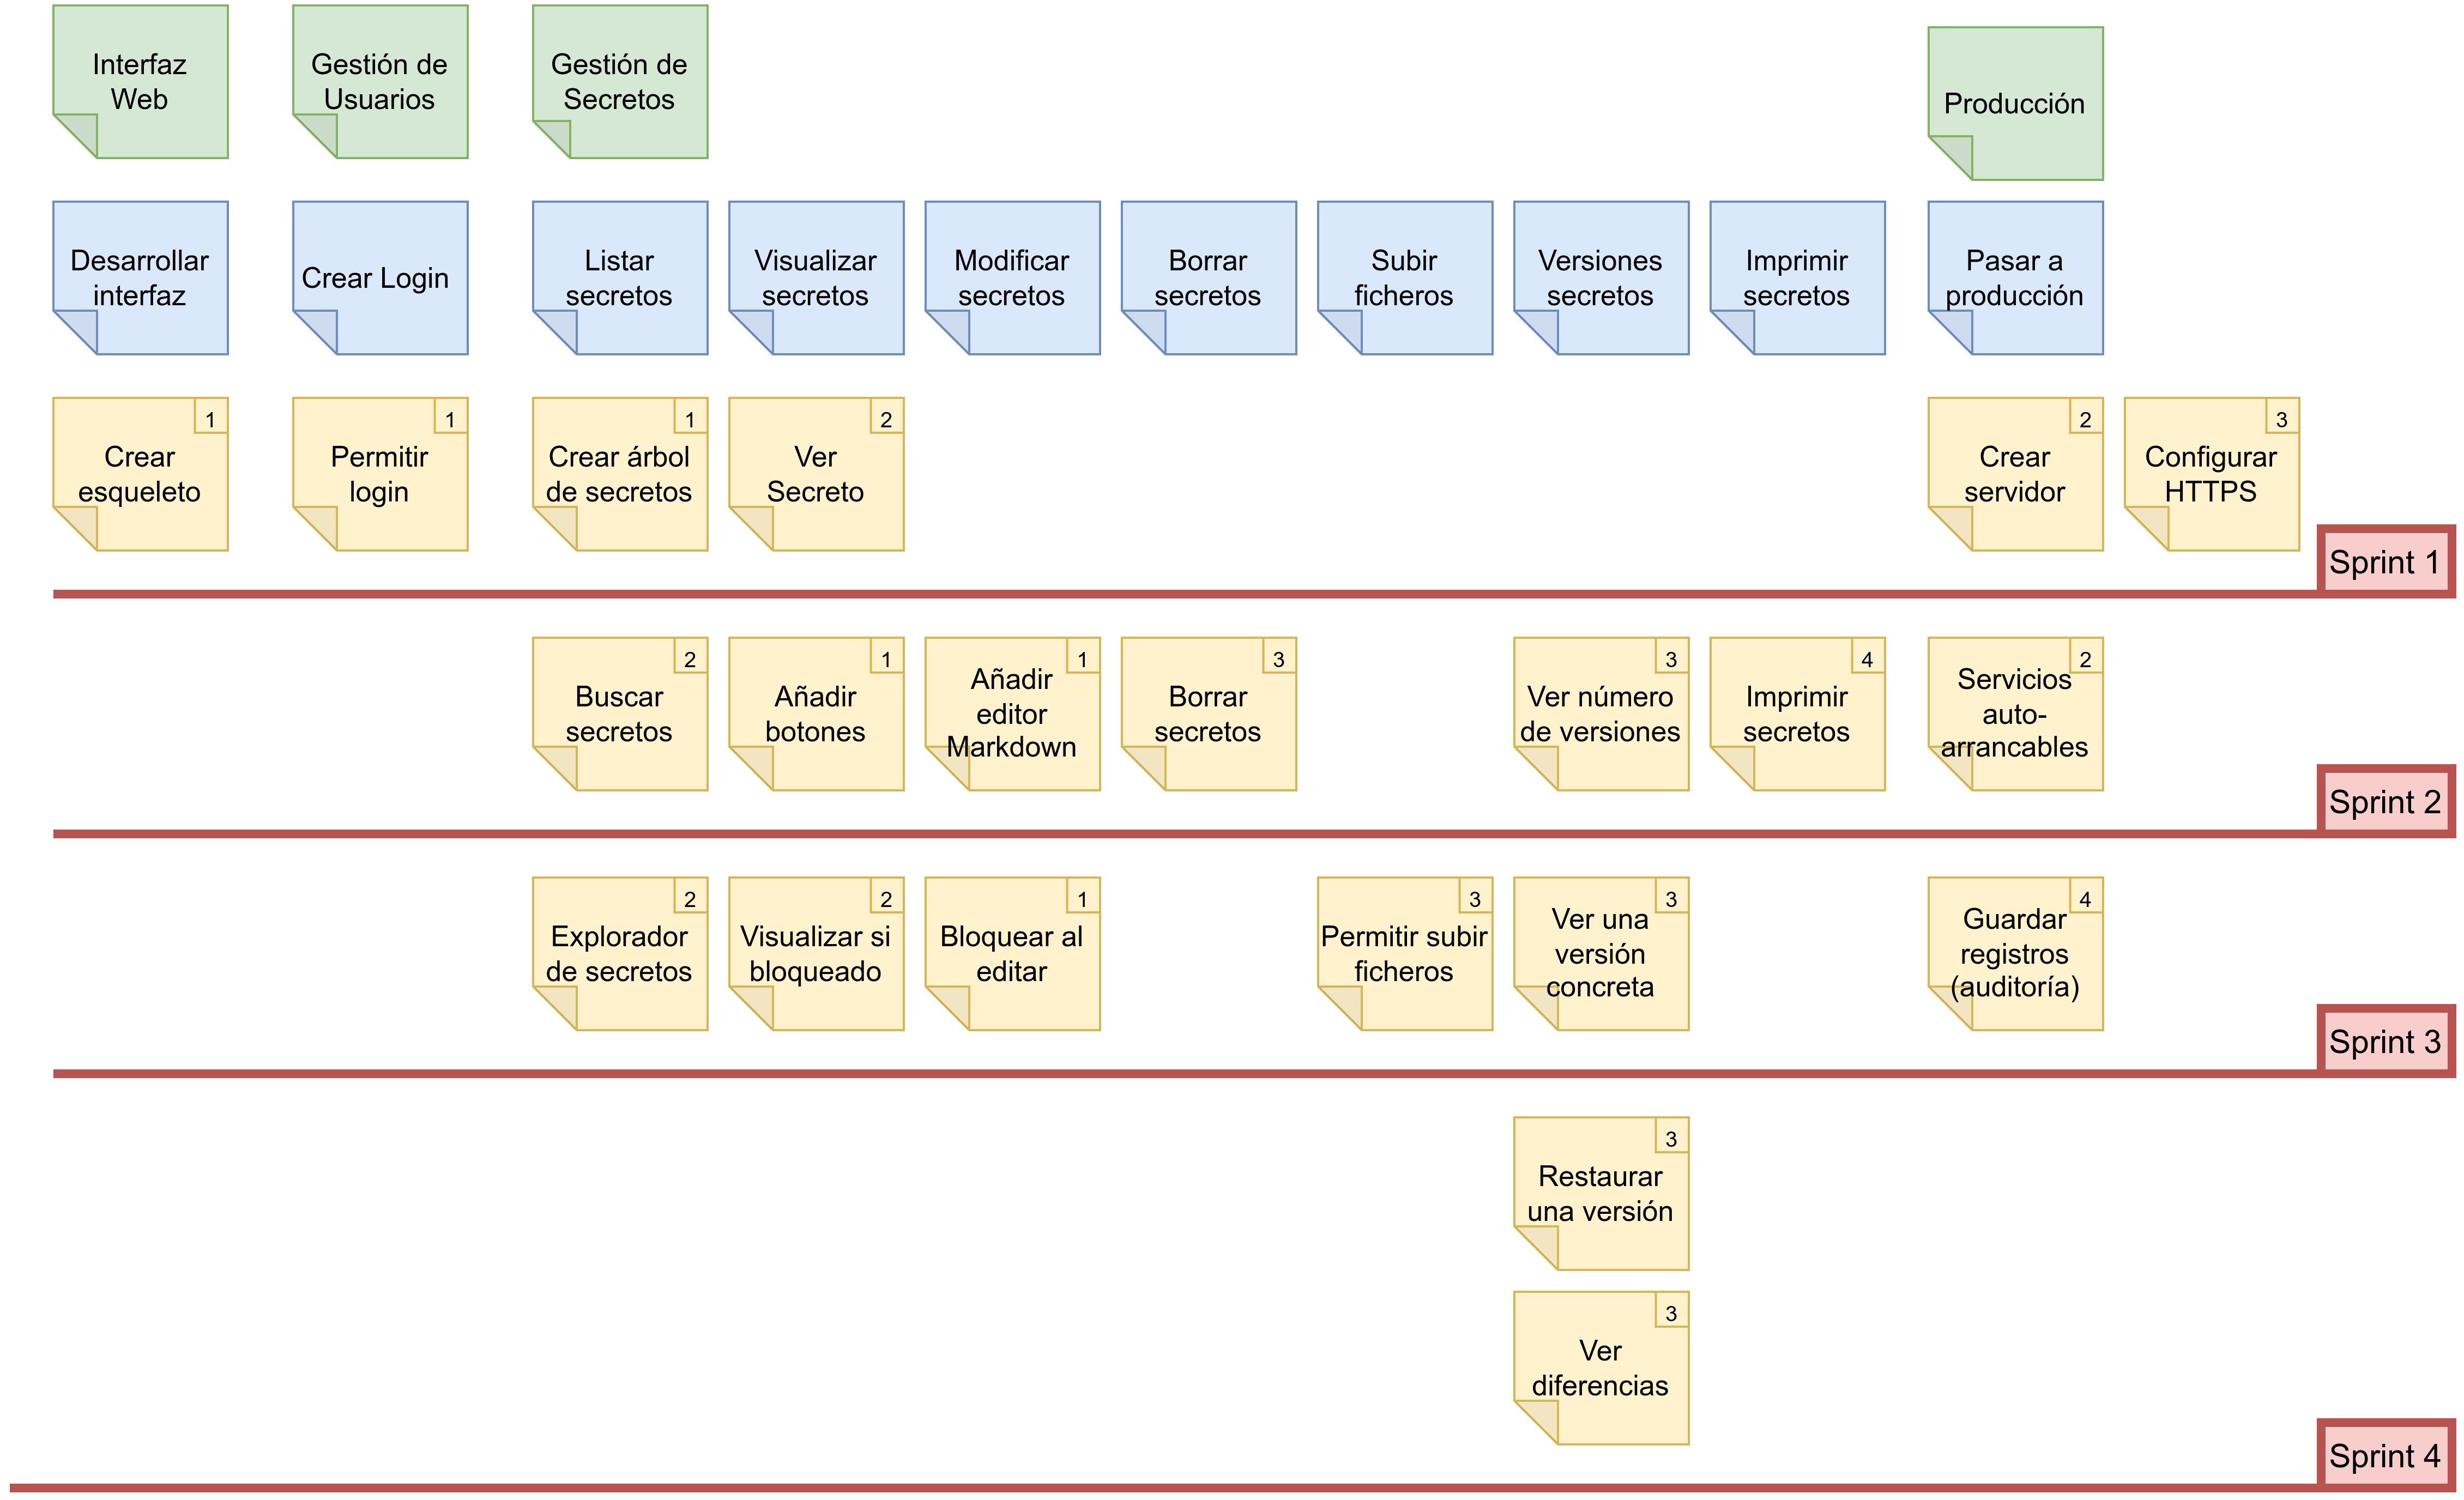
\includegraphics[angle=90,height=\textheight]{img/kanban.png}
    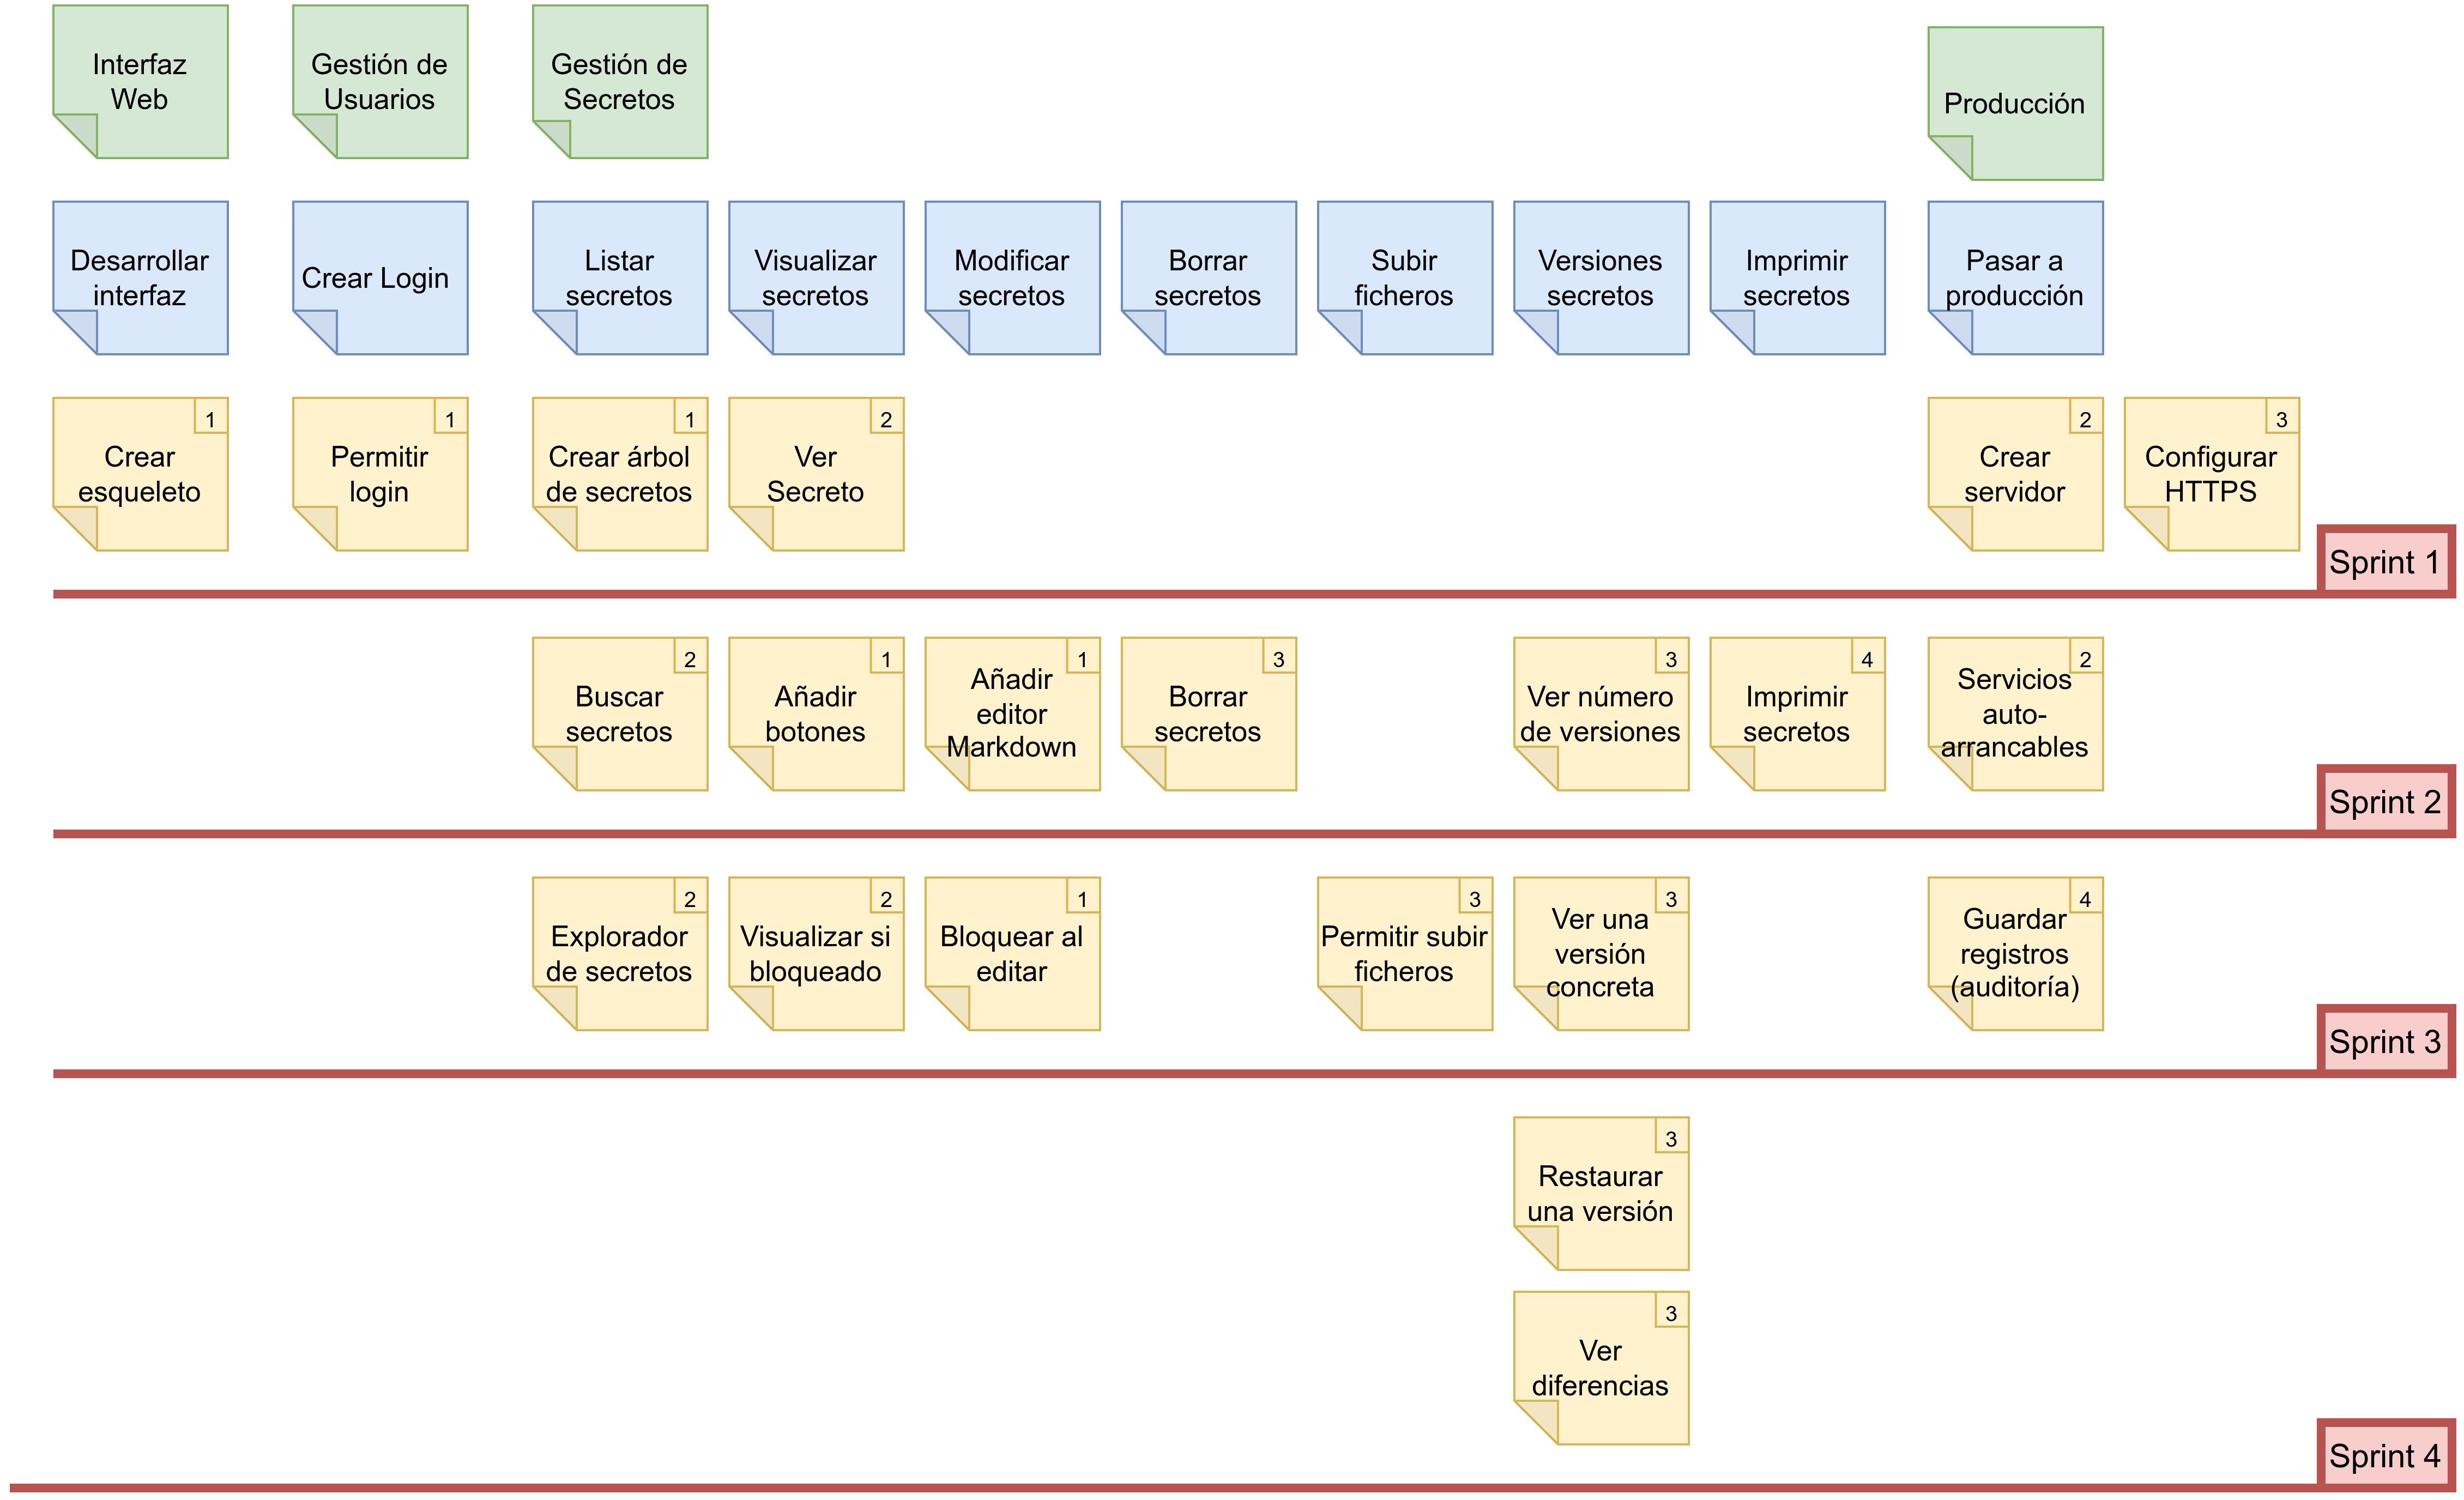
\includegraphics[width=\linewidth]{img/kanban.png}
\end{center}

\chapter{Conclusiones}

La gestión de pro

\end{document}
